\section{Experiments}

For our training and primary evaluation, we utilize multi-hop long-text question answering (QA) tasks, and further conduct evaluations on other various long-text tasks. We select prior long-context methods as baselines to evaluate the long-text extrapolation capabilities of the models by comparing performance changes as the length of the test set data increases.

\subsection{Datasets}

RULER~\cite{hsieh2024ruler} comprises various synthetic tasks with controllable context lengths, making it an ideal benchmark for investigating how model performance varies with increasing context length. 

The Question Answering subset of RULER adapts existing short-context QA datasets for long-context evaluation by embedding golden paragraphs (containing correct answers) within extensive distractor content sampled from the same dataset. This configuration represents a real-world adaptation of the Needle in a Haystack (NIAH) paradigm, where questions serve as queries, golden paragraphs function as needles, and distractor paragraphs constitute the haystack. This task bridges the gap between synthetic evaluation and practical long-context applications, well poised for assessing a model’s ability to locate and extract relevant information from realistic document collections.

We synthesized training samples from the HotpotQA dataset using this methodology. Our synthetic data comprises a total of 200 articles, with an approximate token length of 28K. 

We thoroughly cleaned our dataset by filtering out questions where the Best-Of-2 score is 100\%  without requiring any context for Qwen2.5-7B-Base or Qwen2.5-7B-Instruct. These questions likely represent common knowledge already internalized within the models' memories. Using this method, we processed 80,000 samples from the HotpotQA~\cite{yang2018hotpotqa} training split. Approximately 50\% of the data were filtered out, and from the remaining samples we selected the frist 32,768 samples for further use.

We then applied a similar approach to synthesize 128 samples from the HotpotQA validation set. To further investigate how model performance varies with length, we synthesized test sets with different context lengths using the same questions. The number of articles ranges from 50, 100, up to 6400, corresponding to context lengths of approximately 7K, 14K, and up to 3.5M tokens, respectively.

\subsection{Experimental Setup}

\textbf{Training Details} To maintain comparability with previous work, we choose Qwen2.5-7B-Instruct and Qwen2.5-14B-Instruct as  base models for experiments. We implement the framework for multi-conversation with independent contexts based on verl~\cite{sheng2024hybridflow}. During training, we intentionally limit the model to an 8K context window to highlight its extrapolation capabilities. This 8K-window was allocated as follows: 1024 tokens for the query, 5000 tokens for the context chunk, 1024 tokens for the memory, and 1024 tokens for the output, with remaining tokens reserved for the chat template. Consequently, the model typically requires 5 to 7 conversational turns to process the entire context.

\textbf{Hyperparameters} We use the GRPO algorithm for training, applying a KL factor of 1e-3 and disabling the entropy loss. We employ the AdamW optimizer with a learning rate of 1e-6, scheduled with a constant learning rate with linear warm-up. We use a rollout batch size of 128 and 256 for 7B and 14B models, respectively, and a group size of 16. The ratio of the sample batch size to the backpropagation batch size is set to 16.

\textbf{Model Configuration} We use DeepSeek-R1-Distill-Qwen~\cite{guo2025deepseek}, Qwen-2.5-Instruct-1M~\cite{qwen2.5-1m} and QwenLong-L1~\cite{wan2025qwenlong} as baselines. We follow the official configurations of these baseline models to set context lengths. Specifically, for the Qwen2.5-Instruct-1M series, we further extrapolate the context length to 1M tokens using DCA. For the DeepSeek-R1-Distill-Qwen series and QwenLong, the context length is set to 128K tokens. For the model with 128K context length, the input consists of 120,000 tokens, with an output of 10,000 tokens. For the model with 1M context length, the input is 990,000 tokens, with an output of 10,000 tokens.


\subsection{Main Results}

The main experimental results are reported in \autoref{table:main}. We conduct a comparative analysis of all model performances within the context length ranging from 7K to 896K. Specifically, for the \method model, we extend our evaluation to explore its extrapolation capabilities on ultra-long contexts of 1.75M and 3.5M, assessing how the model generalizes beyond the standard context range.

From these results, we observe that \method exhibits remarkable length extrapolation capabilities with only marginal performance decay as the input context length increases. This demonstrates the effectiveness of the proposed memory mechanism combined with reinforcement learning for handling ultra-long context scenarios.

In contrast, baseline models demonstrate distinct failure patterns even within the context window. The reasoning models (DS-Distill-Qwen series) show rapid performance degradation, while QwenLong-L1 maintains reasonable performance within its training length 60K but experiences substantial degradation afterward. The Qwen2.5-Instruct-1M series models maintains an acceptable performance within 112K tokens. However, their performances deteriorate to zero at 896K tokens, well before reaching their theoretical 1M token capacity. This suggests that despite extended context windows, these models struggle with effective information utilization in ultra-long contexts.



\begin{table}[htbp]
    \centering
    \caption{Main experimental results comparing model performance across various context lengths. All values represent accuracy (\%).}
    \label{table:main}
    \small % Adjust font size if needed
\begin{tabular}{lcccccccccc}
\toprule
\multirow{2}{*}{\textbf{Model}} & \multicolumn{10}{c}{\textbf{Length}} \\
\cmidrule(lr){2-11} 
 & \textbf{7K} & \textbf{14K} & \textbf{28K} & \textbf{56K} & \textbf{112K} & \textbf{224K} & \textbf{448K} & \textbf{896K} & \textbf{1.75M} & \textbf{3.5M} \\
\midrule
QwenLong-L1-32B & 72.66 & 75.00 & 72.66 & 60.94 & 31.25 & 17.19 & 13.28 & 11.72 & N/A & N/A \\
Qwen2.5-Instruct-14B-1M & 60.16 & 60.94 & 50.00 & 57.03 & 50.00 & 37.50 & 8.59 & 0.00 & N/A & N/A \\
Qwen2.5-Instruct-7B-1M & 61.72 & 56.25 & 53.91 & 55.47 & 51.56 & 33.59 & 12.50 & 0.00 & N/A & N/A \\
\midrule
DS-Distill-Qwen-32B & 70.31 & 66.41 & 65.62 & 46.88 & 23.44 & 13.28 & 7.81 & 7.03 & N/A & N/A \\
DS-Distill-Qwen-14B & 64.06 & 64.84 & 57.03 & 40.62 & 14.84 & 8.59 & 3.12 & 6.25 & N/A & N/A \\
DS-Distill-Qwen-7B & 30.47 & 12.50 & 3.12 & 0.00 & 0.00 & 0.78 & 0.00 & 0.00 & N/A & N/A \\
\midrule
RL-\method-14B & \textbf{83.59} & \textbf{82.03} & \textbf{84.38} & \textbf{80.47} & 76.56 & \textbf{81.25} & \textbf{75.00} & \textbf{77.34} & \textbf{76.56} & \textbf{78.12} \\
RL-\method-7B & 82.03 & 79.69 & 78.91 & 77.34 & \textbf{79.69} & 72.66 & 74.22 & 76.56 & 75.78 & 71.09 \\
\bottomrule
\end{tabular}
\end{table}



\subsection{Ablation Study}

\textbf{RL Training}
To investigate the impact of reinforcement learning on the memory mechanism, we conduct further ablation experiments. Our baselines are Qwen2.5-Instruct~\cite{yang2024qwen2} series and Qwen2.5-Instruct models which are equipped with memory mechanism without RL training.

As shown in Figure~\ref{fig:agent-ablation}, vanilla models exhibit severe performance degradation as context length increases, especially after 112K where the inputs are truncated because of the context window. While the model equipped with a memory, without RL training, demonstrates better performance and maintains reasonable performance on tasks exceeding the context length, it still experiences an overall decline in performance as the input length increases.

In contrast, RL-trained models maintain consistently high performance across all context lengths with minimal degradation. This demonstrates that while the memory mechanism provides structural support for long contexts, reinforcement learning is essential for teaching models to properly leverage the memory.

\begin{figure}[h]
    \centering
    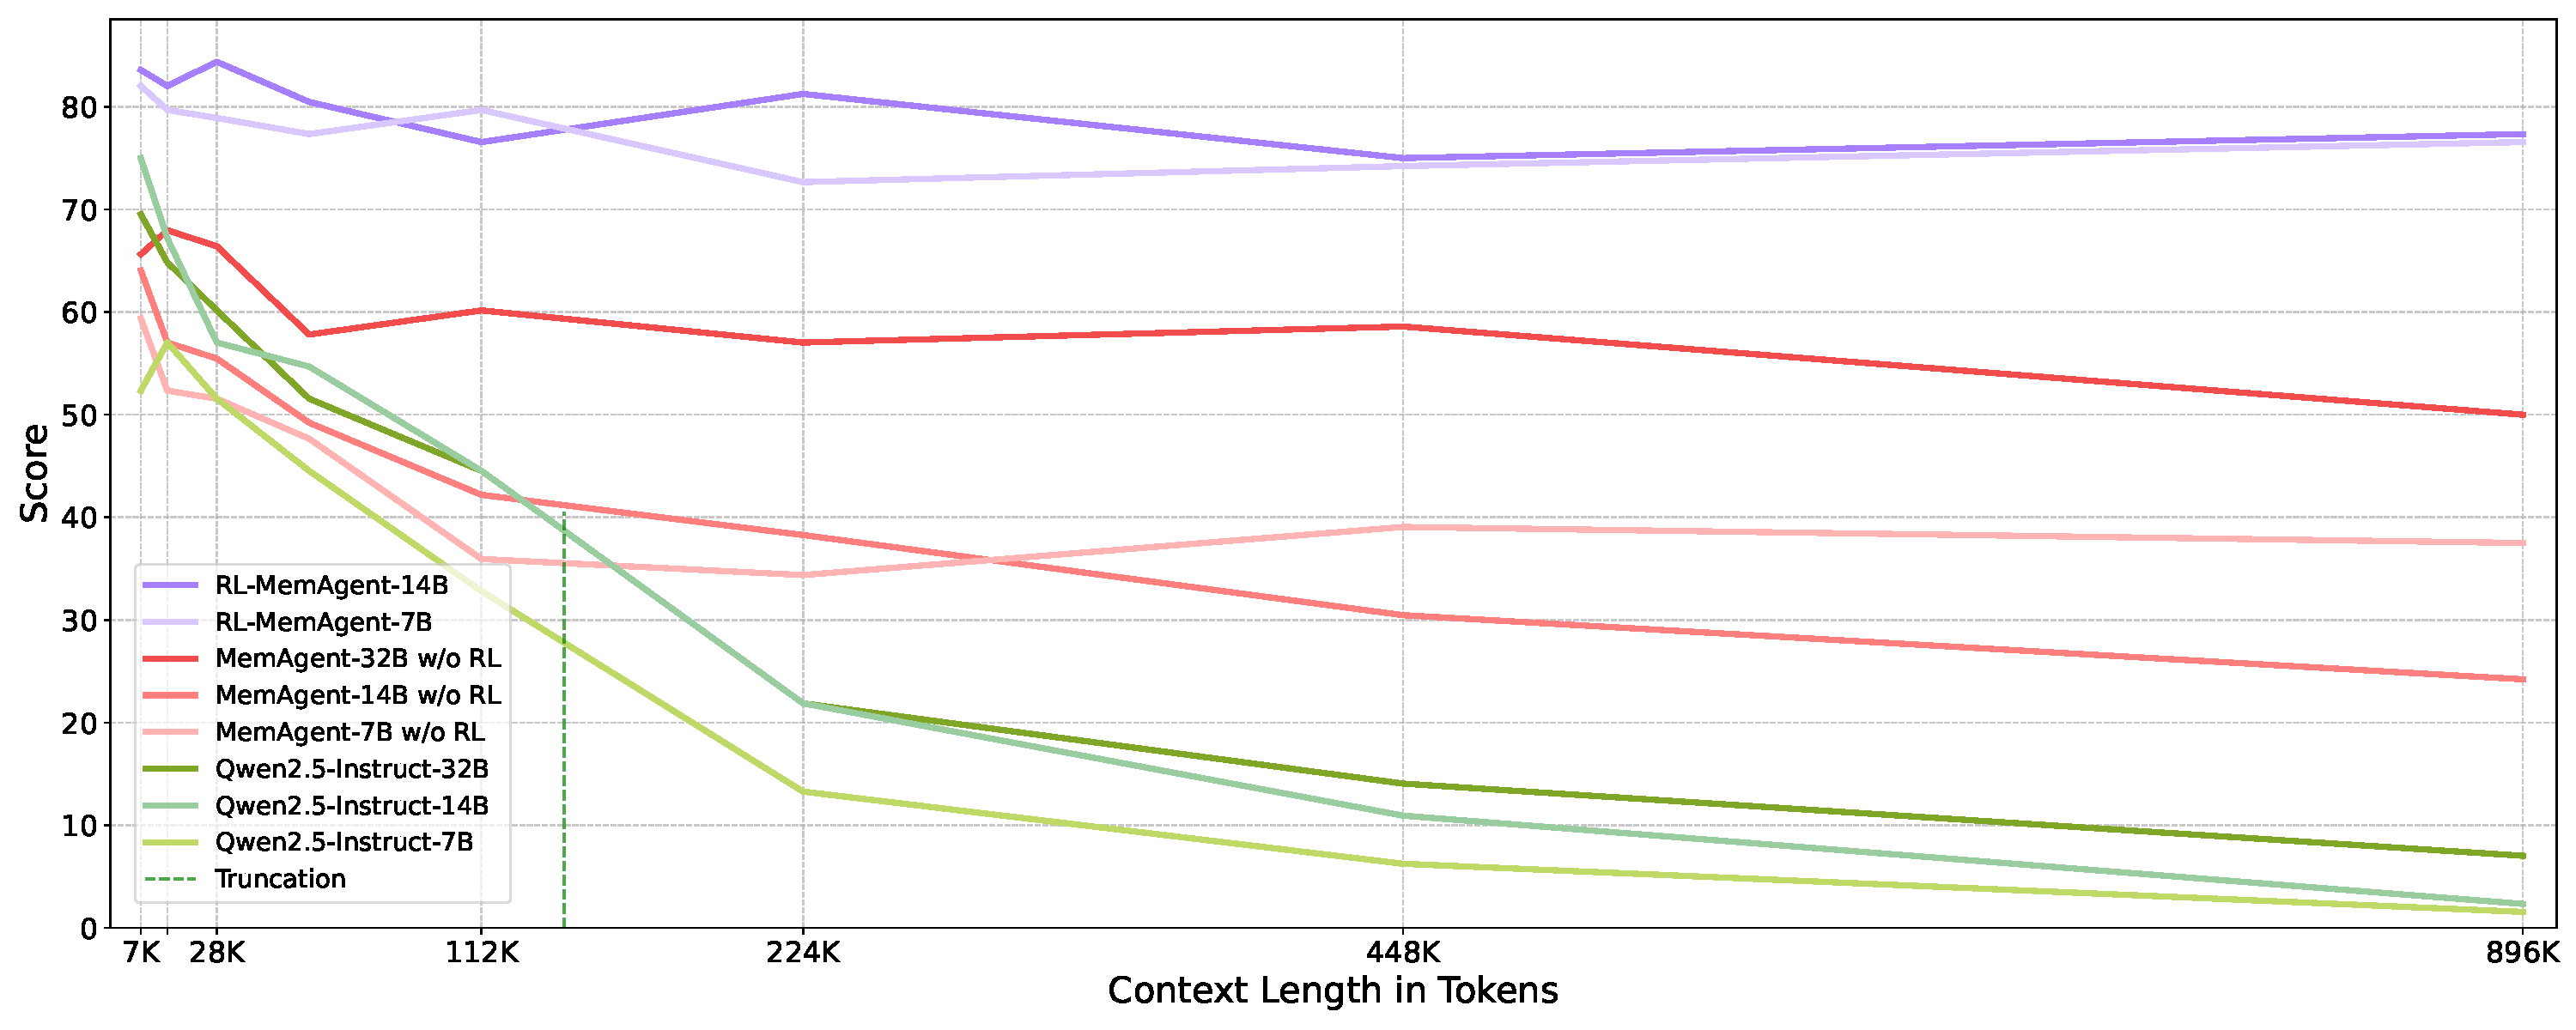
\includegraphics[width=1\linewidth]{figs/ablation.pdf}
    \caption{Ablation study on RULER-HotpotQA comparing models with and without RL training across context lengths from 28K to 896K tokens.}
    \label{fig:agent-ablation}
    \vspace{-10pt}
\end{figure}


\textbf{Out-of-Distribution Tasks}
To evaluate the generalization capabilities of our approach, we conduct comprehensive experiments on the OOD task in RULER benchmark, including \textbf{needle-in-a-haystack variants}, \textbf{variable tracking}, \textbf{frequent words extraction}, and \textbf{question answering} synthesized from SQuAD~\cite{rajpurkar2016squad}. We synthesize context lengths ranging from 8K to 512K tokens for these tasks, except that SQuAD extends only to 256K tokens due to limited document length.

Figure~\ref{fig:ruler-results} presents the performance comparison across different task categories. The results demonstrate that \method maintains consistently superior performance across diverse task types. Particularly, \method-14B achieves over 95\% accuracy on the average RULER tasks in context ranging from 8K to 512K, while \method-7B achieves the best performance, surpassing 32B model without RL training and long-context post-trained models. \method-7B/14B both maintain stable performance on the SQuAD-based QA task, indicating that memorizing ability can generalize beyond training data. In contrast, baseline models show significant degradation beyond 128K tokens across all task categories.

The consistent performance strength across heterogeneous tasks validates that the memory mechanism effectively generalizes to various long-context scenarios rather than overfitting to specific formats. Complete results for all individual RULER tasks are provided in Appendix \ref{sec:OOD}.

\begin{figure}[h]
  \centering
  \begin{subfigure}{0.495\textwidth}
      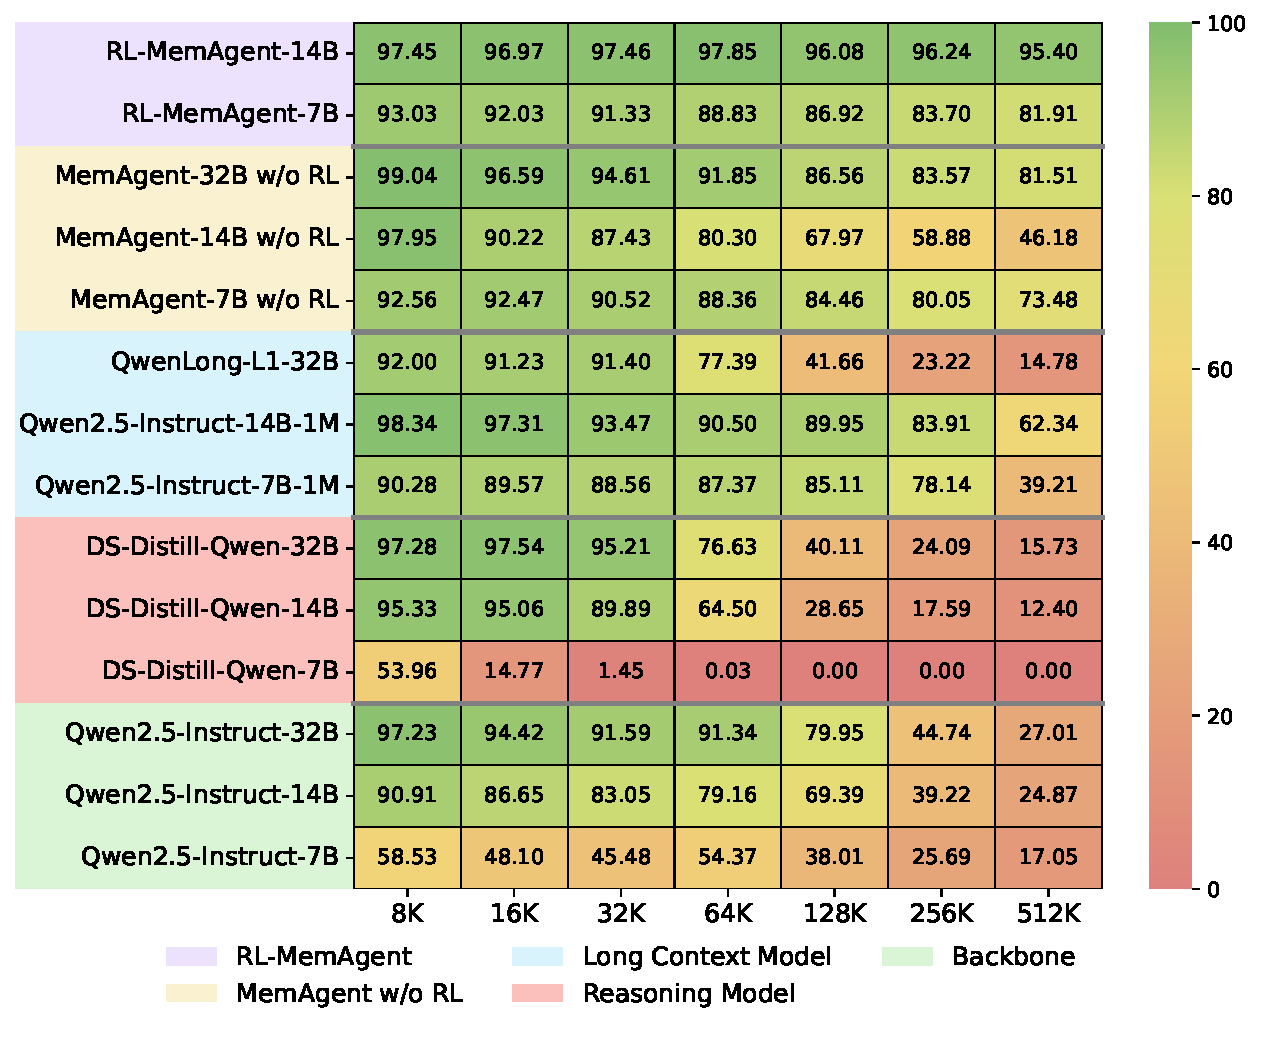
\includegraphics[width=\textwidth]{figs/avg.pdf}
      \caption{RULER average across 10 tasks}
      \label{fig:ruler-avg}
  \end{subfigure}
  \hfill
  \begin{subfigure}{0.465\textwidth}
      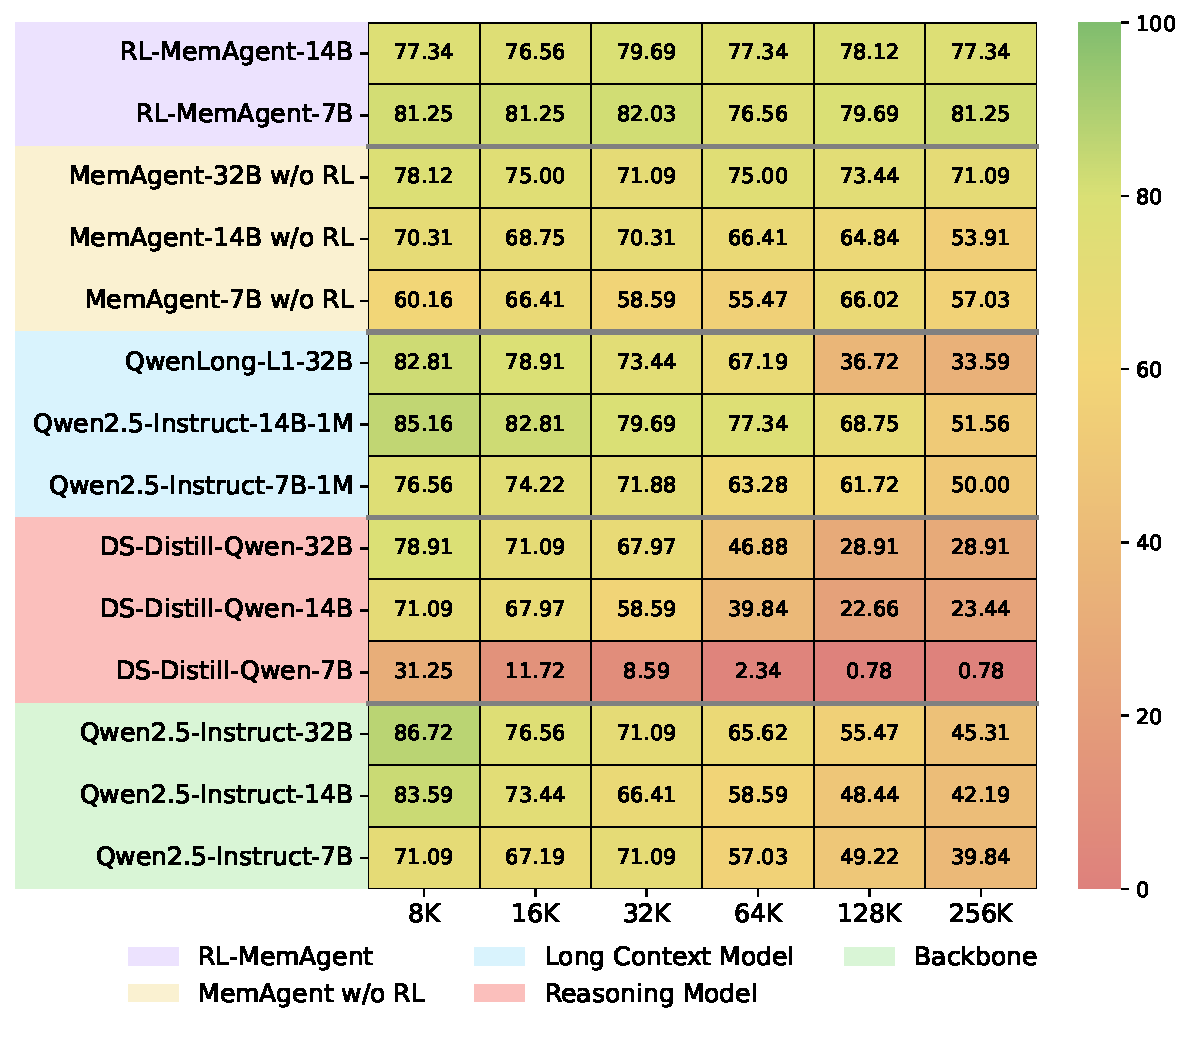
\includegraphics[width=\textwidth]{figs/qa_1.pdf}
      \caption{RULER-QA task from SQuAD}
      \label{fig:ruler-qa1}
  \end{subfigure}
  \caption{Performance heatmaps on RULER benchmark tasks showing accuracy scores across different context lengths (greener indicates better performance). Models are grouped by type on the vertical axis. (a) Average performance across 10 synthetic tasks including needle-in-a-haystack variants, variable tracking, and word extraction. (b) Question answering task synthesized from SQuAD dataset with context lengths up to 256K tokens.}
  \label{fig:ruler-results}
\end{figure}
\subsection{Case Study}

To further illustrate the proposed memory mechanism in detail, we conduct a case study on a generation trajectory of \method-14B. The input question is: \textit{The director of the romantic comedy ‘Big Stone Gap’ is based in what New York city?} This a 2-hop question with the following relevant Wikipedia entries: 

1) \textbf{Big Stone Gap} is a 2014 American drama romantic comedy film written and directed by Adriana Trigiani. 

2) \textbf{Adriana Trigiani} is an Italian American best-selling author of sixteen books, television writer, film director, and entrepreneur based in Greenwich Village, New York City.

In the first round, the model is presented with the entry \textit{Ghost}, which refers to a production team also based in \textit{New York}. The model chooses to retain this potentially useful information for future use. In the second round, no relevant context is provided; nevertheless, the model maintains its agent state, demonstrating robustness against distraction. In the third round, both relevant entries are presented. The model correctly identifies critical information and updates its memory accordingly, leading to the correct answer: \textit{Greenwich Village, New York City}. At this point, the reasoning process is complete. In the remaining rounds, the model’s memory remains unchanged and is used to produce the final response.

\tcbset{colback=seedblue!10!white, colframe=seedblue, width=\linewidth, arc=5mm}
\begin{tcolorbox}
\subsection*{Chunk1}
\vspace{-5pt}

...

Document 20:
Ghost (production team)

Ghost is a Swedish record producing and songwriting team, composed of Ulf Lindström and Johan Ekhé, based in \textit{New York City}.

...
\vspace{5pt}
\subsection*{Memory1}
\vspace{-5pt}
The provided section does not contain any information about the director of the romantic comedy "Big Stone Gap" or their base in New York City. \textbf{However, it does mention a production team called "Ghost" which is based in New York City.} Since the problem is specifically asking about the director of "Big Stone Gap," and there is no direct information about the director in the given section, we cannot infer anything directly related to the problem from the provided text.

Updated memory:
\begin{itemize}
    \item Ghost is a Swedish record producing and songwriting team, composed of Ulf Lindström and Johan Ekhé, based in New York City. They are perhaps best known for writing and producing Swedish singer Robyn's three first studio albums.
\end{itemize}


The problem remains unanswered based on the provided section. Additional information would be needed to determine the director of "Big Stone Gap" and their base in New York City.


\end{tcolorbox}
\tcbset{colback=seedblue!10!white, colframe=seedblue, width=\linewidth, arc=5mm}
\begin{tcolorbox}
\subsection*{Chunk2}
\vspace{-5pt}

...(No relevant document)
\vspace{5pt}
\subsection*{Memory2}
\vspace{-5pt}
\textbf{The provided section does not contain any information about the director of the romantic comedy "Big Stone Gap" or their base in New York City. Therefore, the updated memory remains unchanged with respect to the problem at hand.} The memory still notes that the Ghost record producing and songwriting team is based in New York City, but it does not provide any information about the director of "Big Stone Gap."

Updated memory:
\begin{itemize}
    \item Ghost is a Swedish record producing and songwriting team, composed of Ulf Lindström and Johan Ekhé, based in New York City. They are perhaps best known for writing and producing Swedish singer Robyn's three first studio albums.
    \item The problem remains unanswered based on the provided section. Additional information would be needed to determine the director of "Big Stone Gap" and their base in New York City.
\end{itemize}

\end{tcolorbox}
\tcbset{colback=seedblue!10!white, colframe=seedblue, width=\linewidth, arc=5mm}
\begin{tcolorbox}
\subsection*{Chunk3}
\vspace{-5pt}

...

Document 81:
Big Stone Gap (film)

\textbf{Big Stone Gap} is a 2014 American drama romantic comedy film written and directed by \textbf{Adriana Trigiani} and produced by Donna Gigliotti for Altar Identity Studios, a subsidiary of Media Society.
% Based on Trigiani's 2000 best-selling novel of the same name, the story is set in the actual Virginia town of Big Stone Gap circa 1970s. The film had its world premiere at the Virginia Film Festival on November 6, 2014.

...

Document 96:
Adriana Trigiani

\textbf{Adriana Trigiani} is an Italian American best-selling author of sixteen books, television writer, film director, and entrepreneur based in \textcolor{red}{\textbf{Greenwich Village, New York City}}. 
% Trigiani has published a novel a year since 2000.

...
\vspace{5pt}
\subsection*{Memory3}
\vspace{-5pt}
Updated memory:

\itemize
\item Ghost is a Swedish record producing and songwriting team, composed of Ulf Lindström and Johan Ekhé, based in New York City. They are perhaps best known for writing and producing Swedish singer Robyn's three first studio albums.
\item \textbf{Adriana Trigiani} is an Italian American best-selling author of sixteen books, television writer, film director, and entrepreneur based in Greenwich Village, New York City. Trigiani has published a novel a year since 2000.
\item \textbf{Big Stone Gap} is a 2014 American drama romantic comedy film written and directed by Adriana Trigiani and produced by Donna Gigliotti for Altar Identity Studios, a subsidiary of Media Society. Based on Trigiani's 2000 best-selling novel of the same name, the story is set in the actual Virginia town of Big Stone Gap circa 1970s. The film had its world premiere at the Virginia Film Festival on November 6, 2014.

The director of the romantic comedy "Big Stone Gap" is Adriana Trigiani, who is based in \textbf{\textcolor{red}{Greenwich Village, New York City}}.

\end{tcolorbox}

This trajectory highlights several core capabilities learned by the memory agent: estimating potentially relevant content from query keywords and storing it preemptively, immediately updating memory upon encountering context that matches the query, and remaining unaffected by irrelevant information. Notably, these memory behaviors are not the result of architectural attention mechanisms, but emerge as text generation abilities reinforced through RL.
